We evaluate our design methodology, as applied to BraggNN, and a few NN functional units, against ScaleHLS\cite{ye2021scalehls} and SODA-OPT\cite{9516615}, two state-of-the-art but general purpose DNN compiler to HLS tool flows.
Both tools perform design space exploration but at the cost of high-runtimes and ultimately inferior results \emph{when latency is the only metric}.


\begin{figure}
	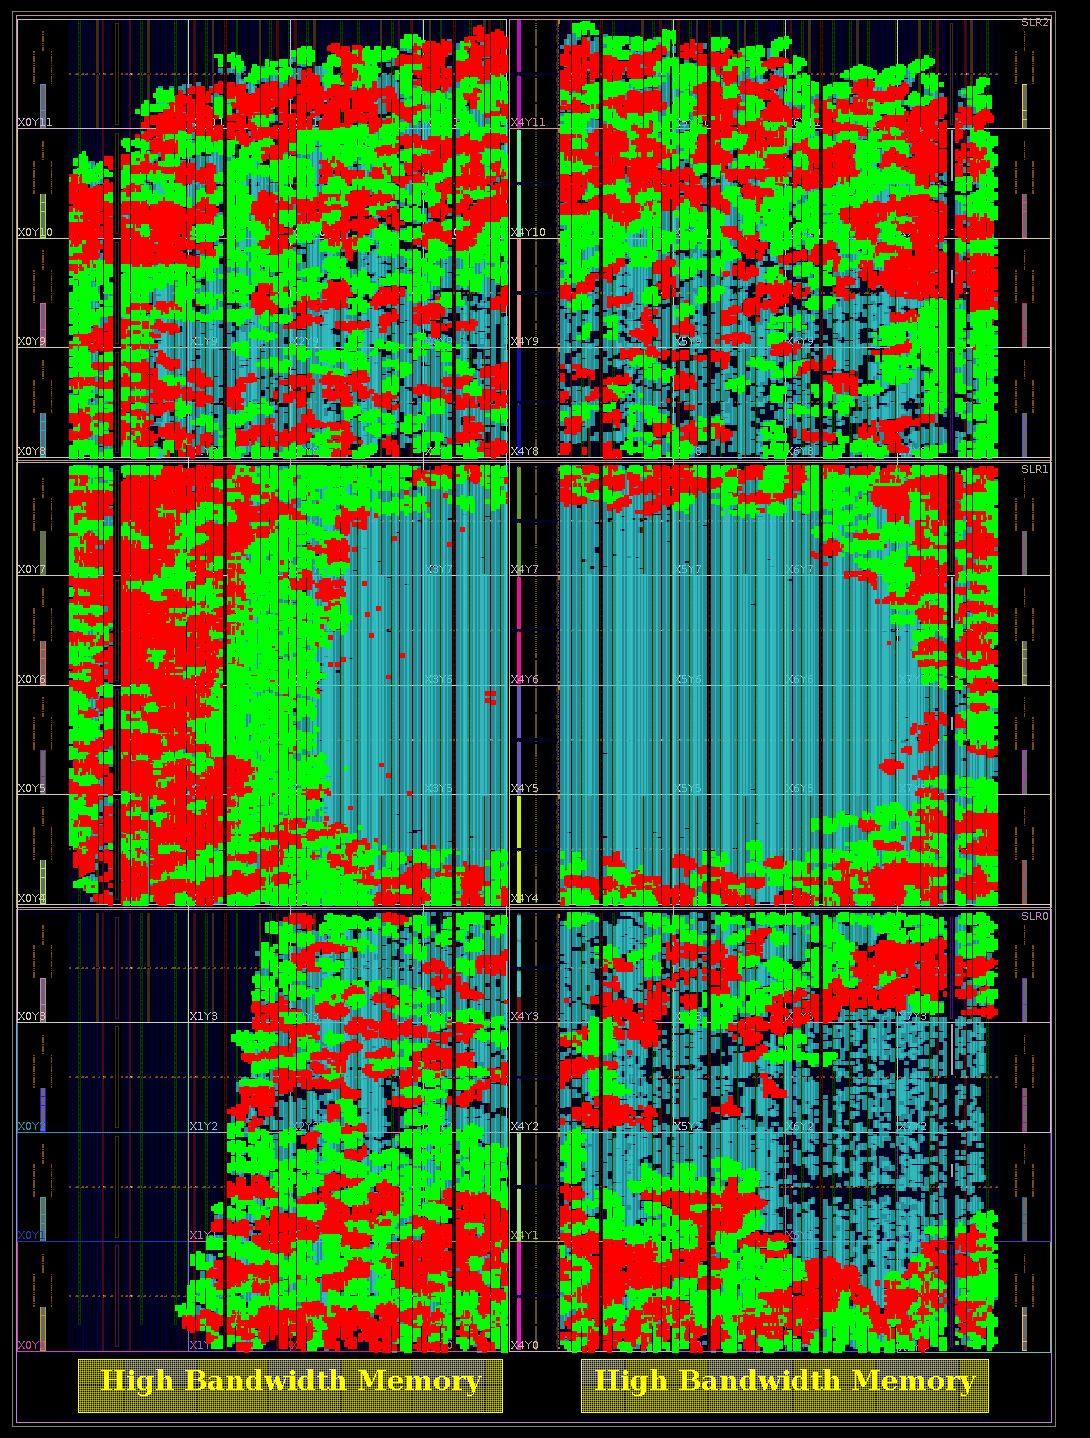
\includegraphics[width=\columnwidth]{figures/placed_braggnn.png}
	\caption{Fully synthesized and placed (on Xilinx Alveo U280) design for BraggNN. \crule[red]{0.25cm}{0.25cm} regions represent \texttt{fmul} leaf cells, while \crule[green]{0.25cm}{0.25cm} regions represent \texttt{fadd} leaf cells.}\label{fig:placed_braggnn}
\end{figure}